\section{Identification des briques logicielles}

%
\subsection{Module d'IA et d'environnement}

Dans ce module, on distingue plusieurs entités~:
\renewcommand{\labelitemi}{$\bullet$}
\begin{itemize}
\setlength{\itemsep}{5pt}
\item L'environnement, espace dans lequel évolue les objets. En pratique, généralement $\mathbb{R}^2$ ou $\mathbb{R}^3$.
\item Les objets, étant de plusieurs types~:
	\begin{enumerate}
	\item Les ressources, que l'on peut affecter à une tâche et qui sont donc mobiles dans l'environnement.
	\item Les tâches, fixes dans l'environnement et qui permettent de modifier un ou plusieurs objectifs.
	\item Les obstacles, fixes dans l'environnement et qui modélisent la structure de l'espace.
	\end{enumerate}
\item L'IA, qui va selon une ou plusieurs stratégies observer l'environnement et prendre des décisions pour résoudre le problème d'affectation.
\item Les contraintes et objectifs, qui permettent de définir des seuils (minimal, maximal, proportion) par rapport à un type de tâche.
\item Les stratégies, qui définissent un déroulement du processus d'affectation (fonction de coût, algorithmes utilisés)
\item Les modèles d'apprentissage et de prise de décision (non étudié ici).
\end{itemize} %\vspace{4mm}

%
\subsection{Module d'indexation spatiale et de partitionnement spatial}

Les entités de ce module sont~:
\begin{itemize}
\setlength{\itemsep}{5pt}
\item Les arbres, servant à stocker l'information spatiale et y accéder rapidemment.
\item Les techniques de construction de ces arbres. Il s'agit principalement d'algorithmes qui sont plus spécifique à chaque structure de données et qui peuvent les améliorer. On peut citer par exemple le Z-order qui permet de construire de manière efficace des Quadtree ou des arbres de Hilbert.
\end{itemize}

%
\subsection{Module d'algorithmes de plus court chemin}

Les entités de ce module sont simplement les algorithmes travaillant sur l'environnement transformé grâce aux techniques d'indexation et partitionnement spatial.

%
\subsection{Module d'affectation}
%TODO
% Passage en paramètre ressources dispo.
% 1. Fonction d'évaluation qui crée matrice
% 2. Algo

%
\section{Cas d'utilisation}

\subsection{Environnement et IA}
\begin{figure}[!h]\centering
   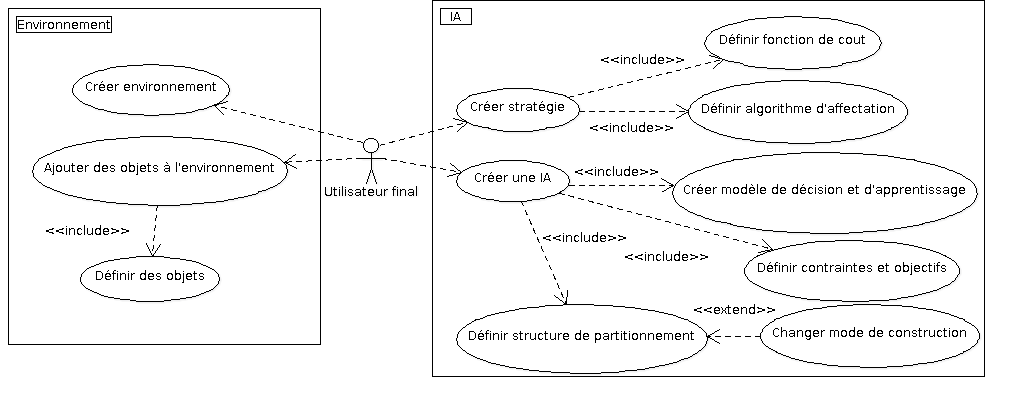
\includegraphics[scale=0.5]{images/uc_main.png}
   \caption{\label{uc_main} Cas d'utilisation généraux}
\end{figure}
\subsection{Ressources}
\begin{figure}[!h]\centering
   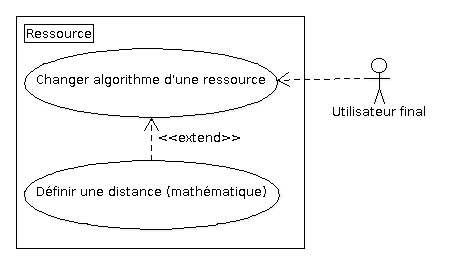
\includegraphics[scale=0.5]{images/uc_ressource.png}
   \caption{\label{uc_main} Cas d'utilisation liés aux ressources}
\end{figure}
\subsection{Framework}
\begin{figure}[!h]\centering
   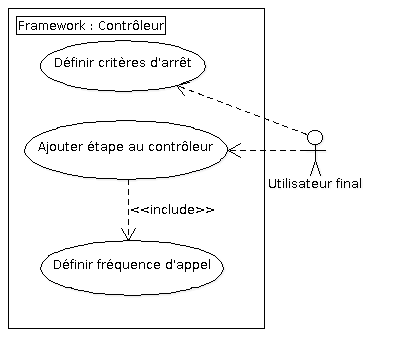
\includegraphics[scale=0.5]{images/uc_framework.png}
   \caption{\label{uc_main} Cas d'utilisation liés au framework}
\end{figure}
%
\section{Scénario}

On peut distinguer plusieurs scénarios pour notre application. Le scénario utilisateur où l'acteur principal est l'utilisateur final, c'est à dire celui qui va utiliser le framework pour résoudre un problème en fonction de son contexte.\\

Des scénarios annexes existent, relatifs aux sous-systèmes du framework et à l’interaction entre ses composants. Le principal est celui qui intervient durant toute la simulation / résolution et dont l'acteur principal est le contrôleur du framework.

%
\subsection{Scénario principal}

\renewcommand{\labelitemii}{$\hookrightarrow$}
\renewcommand{\labelitemiii}{$\circ$}
\begin{itemize}
\setlength{\itemsep}{5pt}
\item L'utilisateur définit ses tâches
	\begin{itemize}
	\setlength{\itemsep}{2pt}
	\item Définition des contraintes liées à chaque tâches
	\item Définition des contraintes générales (applicables à chaque tâches ou inter-tâches)
	\end{itemize}
\item L'utilisateur définit l'environnement
	\begin{itemize}
	\setlength{\itemsep}{2pt}
	\item Définition de l'espace (dimensions, frontières)
	\item Définition des objets statiques (obstacles)
	\item Définition des objets dynamiques
		\begin{itemize}
		\item Définition des ressources
			\begin{itemize}
			\item Définition d'une fonction de coût
			\end{itemize}
		\item Définition des emplacements de travail
			\begin{itemize}
			\item Observation de l'emplacement par un type de tâche
			\end{itemize}
		\end{itemize}
	\item Paramétrage de l'environnement
		\begin{itemize}
		\item Délais de mise à jour
		\end{itemize}
	\end{itemize}
\item Création des stratégies
	\begin{itemize}
	\setlength{\itemsep}{2pt}
	\item Définition de la fonction de coût globale
	\item Définition de l'algorithme d'affectation
	\end{itemize}
\item Création de l'IA
\item Définition du modèle de décision et d'observation
\item Définition de l'algorithme de partitionnement de l'espace
\item Définition de l'algorithme d'indexation des objets dynamiques
\item Ajout des stratégies
\item Paramétrage de l'IA
	\begin{itemize}
	\item Délais entre chaque cycle \og observation – apprentissage – prise de décision - affectation \fg
	\end{itemize}
\item Lancement de la simulation / résolution par le contrôleur du framework.
\end{itemize} %\vspace{4mm}


\subsection{Scénarios annexes}

\begin{enumerate}
\setlength{\itemsep}{8pt}
%
\item Initialisation
\item[]
	\begin{itemize}
	\setlength{\itemsep}{5pt}
	\item Partionnement de l'espace
	\item Indexation sous forme d'arbres %Listage
		\begin{itemize}
		\item Des ressources
		\item Des emplacements de travail
		\item Des tâches
		\item Des obstacles
		\end{itemize}
	\end{itemize}
%
\item Déroulement de la simulation / résolution
\item[]
	\begin{itemize}
	\setlength{\itemsep}{5pt}
	\item Le contrôleur principal appelle le contrôleur de l'IA si la contrainte de temps est respectée
	\item Le contrôleur de l'IA~:
		\begin{itemize}
		\setlength{\itemsep}{2pt}
		\item Observation du monde
		\item Apprentissage (non étudié ici)
		\item Prise de décision (non étudié ici - peut être effectué manuellement par l'utilisateur)
		\item Affectation
			\begin{itemize}
			\item Appelle un algorithme de réaffectation pour les ressources disponibles
			% Passage en paramètre des ressources disponibles
			% 1. Fonction d'évaluation
			% 2. Algo en lui-même
			\end{itemize}
		\end{itemize}
	\item Le contrôleur principal appelle le contrôleur de l'environnement si la contrainte de temps est respectée
	\item Le contrôleur de l'environnement~:
		\begin{itemize}
		\item Mise à jour des objets dynamiques (Ressources / Unités \ldots)
		\end{itemize}
	\item Le contrôleur principal met à jour l'affichage
	\item La boucle recommence tant que les conditions sont respectées
	\end{itemize}
%
\item Observation du monde
\item[]
	\begin{itemize}
	\setlength{\itemsep}{5pt}
	\item Observation des contraintes / objectifs
	\item Observation de l'environnement~: les objets dynamiques
		\begin{itemize}
		\setlength{\itemsep}{2pt}
		\item Ressources
		\item Emplacements de travail
		\end{itemize}
	\end{itemize}
%
\item Affectation
\item[]
	\begin{itemize}
	\setlength{\itemsep}{5pt}
	\item Algorithme d'affectation appelé, exemple~:
		\begin{itemize}
		\setlength{\itemsep}{2pt}
		\item Méthode hongroise
		\item Recherche des voisins les plus proches
		\end{itemize}
		\item %TODO à préciser - ade
	\item Attribution d'une tâche à chaque ressource
	\end{itemize}
\end{enumerate} %\vspace{4mm}

%
\section{Diagramme de séquence}
%TODO

%
\section{Modélisation des entités}

\subsection*{Tâche}

Une tâche est définie par une représentation numérique. Ne doit pas être confondue avec l'emplacement de travail (TaskSpot) qui est un objet concret de l'environnement qui peut modifier la  tâche.

\subsection*{Contraintes}

Une contrainte est une assertion et sera modélisée sous forme de foncteur renvoyant vrai ou faux.
Il existe plusieurs types de contraintes ayant plusieurs fonctionnement. Chacune possède une priorité qui pourra représenter soit un ordre de traitement par l'IA ou une pénalité lors de l'évaluation. \\

\textbf{Note}~: Il serait intéressant de pouvoirs détecter les contraintes impossibles à tenir en fonction de l'environnement ou tout simplement parce que deux contraintes s'opposent. Le problème de satisfaction de contraintes est à lui tout seul un problème NP-difficile dans la plupart des cas.\\
\indent On supposera durant ce projet que ce point ne pose pas de soucis et que l'utilisateur n'entrera pas des contraintes qui pourront amener le système à se bloquer ou à ne pouvoir satisfaire l'ensemble des contraintes dans un temps raisonnable.\\
\indent Par la suite il pourra néanmoins être intéressant de proposer des algorithmes de déduction de contraintes et de résolution du problème CSP (Constraint satisfaction problem).

\subsection*{Contraintes de seuils}

Une contrainte de seuil (appliquée à une tâche) est composée d'un opérateur $\leq$ ou $\geq$, et d'une valeur numérique.\\
\indent Ces contraintes possèdent deux fonctions de callback qui doivent se déclencher lorsque l'on franchi le seuil défini, d'un côté et de l'autre (ie, cela implique de garder en mémoire la valeur lors de la vérification précédente).\\
\indent Optionnellement, on peut définir un intervalle de tolérance non nécessairement symétrique.

\subsection*{Contraintes de de proportionnalité}

Défini une relation de proportionnalité entre 2 ou plusieurs tâches.
On peut imaginer par exemple vouloir 30 \% de pierres contre 70 \% d'or dans le cadre d'un jeu de statégie.\\
\indent Là encore, on peut définir de manière optionnelle un intervalle de tolérance et deux fonctions de rappel qui seront appelées en cas de changement de statut de la contrainte (passage du respect ou non respect et inversement).

\subsection*{Contraintes personnalisées}

Une contrainte personnalisée est une contrainte modélisée par une fonction renvoyant un booléen~: vrai si la condition est vérifiée, faux sinon.
Elles servent à exprimer des contraintes diverses sur les tâches mais aussi sur d'autres éléments de l'environnement en fonction du problème de l'utilisateur.\\

Ces contraintes portent également deux fonctions de rappel pour le changement de statut de la contrainte.

\subsection*{Système de contraintes}
Il s'agit d'un système comprenant les tâches ainsi que les contraintes. Les  tâches / contraintes sont potentiellement indépendantes de l'IA qui va résoudre le problème puisqu'elles appartiennent au problème lui même.\\

Ainsi le but du système de contraintes de centraliser les tâches et les contraintes pour en faciliter l'accès par l'utilisateur et l'IA.\\
\indent Le système pourra également proposer des méthodes de résolution du CSP évoquées plus haut.
De plus, le système impose une représentation homogène pour l'ensemble des tâches.\\

{\color{blue}{
\noindent Schéma de classes du système.\\
Schéma d’interaction avec l'utilisateur.\\
Schéma d’interaction avec l'IA.
}}

\subsection*{L'environnement}

Il est composé d'un espace au sens mathématique, ainsi que de 3 types d'objets~: les obstacles, les points de travail et les ressources. Il a donc principalement un rôle de conteneur.\\

\'Etant donné que la création de l'environnement peut très vite devenir complexe, un design pattern builder est envisagé, permettant par exemple de charger un fichier d'environnement depuis différents types de fichiers.
Ce sera d'ailleurs le cas pour l'application d'exemple.\\\\

L'environnement est à la fois un observateur et un observable. Il est observé par l'IA et observe les objets dynamiques qu'il contient. Ainsi il s'agit d'un médiateur entre les objets qu'il contient et l'IA.

\subsection*{L'espace}

L'espace est simplement défini par un nombre de dimensions et le type de ses coordonnées.
Il contient également les limites de l'espace. L'espace peut donc être imaginé comme un parallélotope droit.

\subsection*{Les coordonnées}

Les coordonnées permettent de localiser l'ensemble des objets dans l'espace. Elles présentent deux caractéristiques~: le nombre de composantes et le type de ces composantes. Il s'agit d'un vecteur stockant $n$ composantes d'un type numérique.

\subsection*{Les objets}

Les objets évoluent dans l'environnement et plus particulièrement dans l'espace qu'il contient. Ainsi, tous les objets possèdent des coordonnées qui doivent être du même type que ceux de l'espace considéré.\\
\indent Il existe deux types d'objets (pour le moment)~: les objets statiques et les objets dynamiques. Chacun de ces deux types donnent lieu à une hiérarchie d'objets.\\

Tous les objets implémentent une géométrie qui permettra d'effectuer des calculs de collision selon diverses techniques. Par exemple on peut définir un objet par un polygone convexe, un polygone quelconque, un carré, un cercle. Chaque représentation à ses avantages et inconvénients sur les méthodes de collisions~: algorithme du point dans un polygone (convexe), Bounding-Box, rayon de collision, etc.\\

Tous les objets possèdent également une fonction update qui sert à mettre à jour leur état interne régulièrement.

\subsection*{\textbullet ~Les objets statiques}

Il s'agit des objets de l'environnement qui ne peuvent pas bouger. Leur intérêt principal est de définir des obstacles dans l'espace, bloquant le passage aux ressources.\\

\textbf{$\hookrightarrow$ Les obstacles}\\

Il s'agit du seul objet statique concret dont nous avons perçu l’intérêt pour l'instant. Il est là pour modéliser, comme son nom l'indique, un obstacle dans l'espace.

\subsection*{\textbullet ~Les objets dynamiques}

Ce sont des objets qui sont capables de bouger dans l'espace.\\

\textbf{$\hookrightarrow$ Les ressources}\\

Elles représentent des objets dont l'IA dispose pour pouvoir les affecter à diverses tâches en vu de satisfaire les contraintes du système de contraintes. Il s'agit encore d'une classe abstraite dont le but est de clarifier l'architecture des objets. On retrouvera différents types de ressources ayant des comportements différents.\\

Ainsi on peut imaginer une ressources qui n'est pas réaffectable lorsqu'elle commence une tâche qui lui est donnée par l'IA, on peut imaginer une ressource qui n'accepte qu'un seul type de tâche, etc. Toutes ses variantes dépendent du problème et seront rajoutées à mesure que le besoin s'en fera sentir.\\
\indent Dans notre cas on n'envisagera qu'une unité simple qui pourra être réaffectée n'importe quand, et une unité qui ne pourra pas être réaffectée.\\

\textbf{$\hookrightarrow$ Les emplacements de travail}\\

Ce sont les représentations physiques d'une tâche. C'est à dire des objets qui vont pouvoir modifier une tâche (son \og compteur \fg ) en fonction de certaines conditions.\\
\indent Ainsi, ce sont des observateurs d'une tâche particulière qu'elle notifie en cas de changement.\\

Là encore, on peut imaginer beaucoup de variantes~: des emplacements temporaires – l'emplacement est détruit au bout de tant de temps d'utilisation, des emplacements avec un compteur – l'emplacement se détruit après tant d'utilisation, etc.

\subsection*{Les politiques de chevauchement}

Les objets sont paramétrés par une politique de chevauchement~: certains objets peuvent ne pas en chevaucher d'autres.\\
\indent Il s'agit concrètement d'un entier qui permet de définir une priorité sur le chevauchement. Un objet ne peux pas surpasser un objet ayant une valeur plus haute que la sienne.\\
\indent Des constantes sont prévues pour définir des objets \og fantômes \fg ~et des objets que l'on ne peut pas chevaucher, comme les obstacles par exemple.

\subsection*{Les fonctions de coûts}

Il existe deux types de fonctions de coûts~: les fonctions locales et les fonctions globales. La première est propre à l'évaluation d'une ressource par rapport à un emplacement de travail.
La fonction de coût global qui évalue à un instant donné la qualité de la situation observable par l'IA. Elle est très dépendante du problème et de la stratégie adoptée. Il peut s'agir d'une simple somme des distances des ressources par rapport aux tâches, mais on peut également vouloir prendre en compte la satisfaction des contraintes, ou les tâches en cours avec un poids important, etc.
Elle servira donc plus pour le modèle d'apprentissage, mais comme ce point n'est pas abordé durant ce projet, il s'agira plus d'une fonction annexe ou indicatrice.\\

L'implémentation est très libre et souple au vu de ce que le C++ permet de faire, surtout avec le nouveau standard.

\subsection*{Les stratégies}

Il s'agit d'une manière de résoudre le problème d'affectation pour satisfaire les contraintes. Elle comporte une manière d'évaluer la situation (fonction de coût globale), un algorithme d'affectation et une fonction de coût locale (manière d'évaluer une ressource selon ces caractéristiques).\\\\

Une stratégie très simple consiste à ne traiter la satisfaction que d'une contrainte à la fois. Il s'agira de la seule stratégie que nous implémenterons.

\subsection*{L'IA}

Il s'agit d'un conteneur de stratégies qui sont organisées selon un modèle (couple d'un modèle de décision et d'observation).\\
\indent L'IA défini également un algorithme de partitionnement spatial et un algorithme d'indexation.
Pour pouvoir plus facilement traiter le problème d'affectation, l'IA possède également 3 structures de données qui indexent la topographie de l'espace (donc les objets statiques), les tâches et les ressources à partir des conteneurs basiques de l'environnement.

\subsection*{Arbres}

Utilisés pour indexer les objets, pour partitionner l'espace. On retrouve beaucoup d'arbres différents ayant chacun leurs avantages et désavantages. En voici une liste assez complète qui pourront être implémentés par la suite~:
\begin{itemize}
\item AtlasGrid
\item R-tree
\item Quadtree
\item Octree
\item BSP
\item KD-tree
\item implicit KD-tree
\item vantage KD-tree
\item R+-Tree
\item R*-Tree
\item X-Tree
\item M-Tree
\item Hilbert R-Tree
\item UB-Tree
\end{itemize}

\section{Architecture du framework}

Cette section s'attele à décrire l'architecture globale du framework~:

\subsection*{Contrôleur}

Le contrôleur principal gère le déroulement globale de la simulation. Il s'agit d'une boucle principale avec des critères d'arrêt définis par l'utilisateur (nous proposerons un critère temporel).\\
\indent La boucle principale va effectuer en permanence les même actions, dans le même ordre. Ces actions sont des appels à des contrôleurs locaux ou des actions définis par l'utilisateur parce qu'il en a besoin dans son application~: interception et traitement des entrées claviers, affichage \ldots \\
\indent Par défaut, seules deux actions sont présentes: l'appel au contrôleur local de l'IA et au contrôleur local de l'environnement.\\

Ces actions seront modélisés sous forme d'un deque de fonctions à appeler dans l'ordre. Chaque fonction sera assortie d'un délais d'activation~: toutes les 100ms par exemple.

\subsection*{Logger}
Un logger est absolument nécessaire pour un framework afin de repérer le déroulement du flux d'exécution et localiser d'éventuel(s) problème(s) ou simplement visualiser le processus de calcul. C'est d'ailleurs très utile pour faire des tests unitaires ou d'intégration.\\
\indent Nous mettrons en place un logger sous forme de Design Pattern Chaine de Responsabilité. Chaque maillon de la chaîne sera un logger avec un niveau de log différent (DEBUG, INFO, ERROR \ldots ) et le message transite de maillon en maillon jusqu'à ce que le bon niveau soit atteint.\\
\indent On pourra utiliser une sérialisation dans un fichier texte ou non.\\

Il existera une instance statique du logger pour permettre une utilisation globale. On n'utilisera pas de DP Singleton d'une part parce qu'il est très dur à rendre thread-safe et d'autre part parce pour une raison ou une autre, l'utilisateur final trouvera peut être une utilité à avoir plusieurs loggers.

\subsection*{Le modèle multi-thread}
Nous n'implémenterons pas le modèle multithread pour des raisons de temps mais nous le rendrons facilement intégrable, notamment avec le fonction du contrôleur principal. En effet, les actions du contrôleur sont, normalement, toutes indépendantes et peuvent donc être lancées en parallèle.\\

Pour rendre l'application thread-safe à un niveau de granularité plus fin, on utilisera le paramétrage par politique qui permettra de découpler totalement le modèle multi-thread du reste et d'activer / désactiver le support multi-thread à la volée.

\subsection*{Les observateurs / observables}
Le design pattern Observateur occupe une place importante notamment lors de la récupération d'information sur l'environnement par l'IA mais également par la notification de mise à jour de plus petites entités au sein de l'environnement (les objets). C'est pourquoi nous avons imaginés deux types de politiques liées à l'observation : une politique active et une politique passive.

\subsubsection{Politique active}

La politique active est le comportement classique lorsque l'on parle du patron Observateur. Dès qu'un changement apparaît sur un observé, il notifie l'observateur qui s'est abonné aux observés.\\
On retrouve ce comportement au niveau du couple Emplacement / Tâche où l'emplacement, sous certaines conditions, va notifier la tâche qui devra se mettre à jour.

\subsubsection{Politique passive}

La politique passive consiste pour l'observé à simplement changer son état indiquant qu'il a changé et préparer le message qui doit être transmis à l'observateur. C'est donc l'observateur qui est actif et va explicitement demander la notification d'état et récuperer les messages des observables qui ont indiqués qu'ils étaient modifiés.\\\\
Ce comportement apparaît par exemple au niveau de l'observation de l'environnement par l'IA. L'IA va périodiquement choisir de regarder l'état de l'environnement.

\section{Diagramme de classes}
\subsection{Algorithmes}
\begin{figure}[!h]\centering
   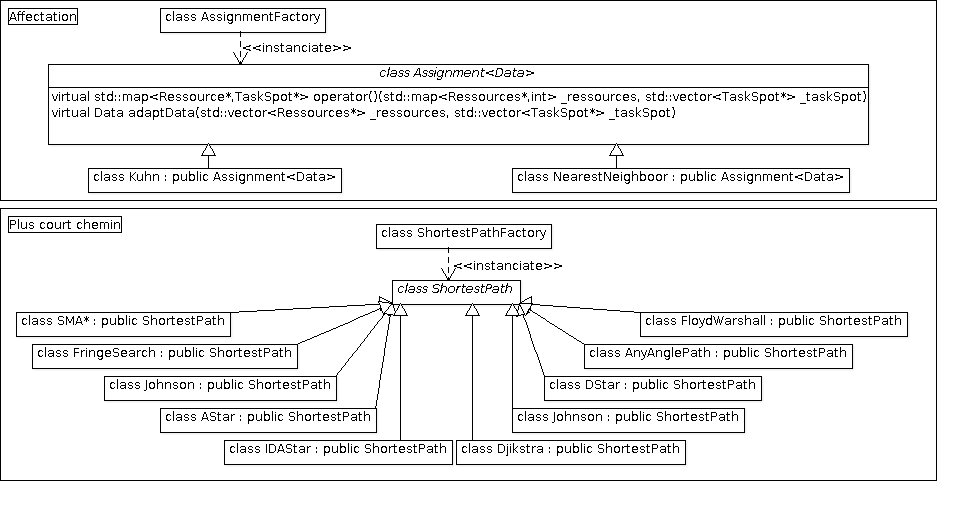
\includegraphics[scale=0.5]{images/c_algo.png}
   \caption{\label{c_algo} Diagramme de classes des algorithmes}
\end{figure}

\subsection{Arbres}
\begin{figure}[!h]\centering
   \includegraphics[scale=0.5]{images/c_arbre.png}
   \caption{\label{c_arbre} Diagramme de classes des arbres}
\end{figure}

\subsection{Framework}
\begin{figure}[!h]\centering
   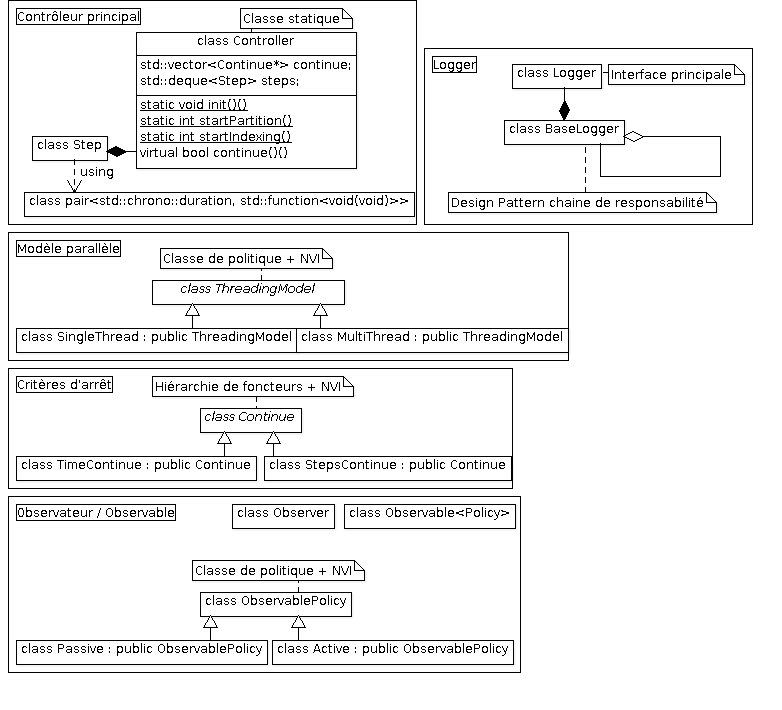
\includegraphics[scale=0.5]{images/c_framework.png}
   \caption{\label{c_framework} Diagramme de classes du framework}
\end{figure}

\subsection{IA \& Contraintes}
\begin{figure}[!h]\centering
   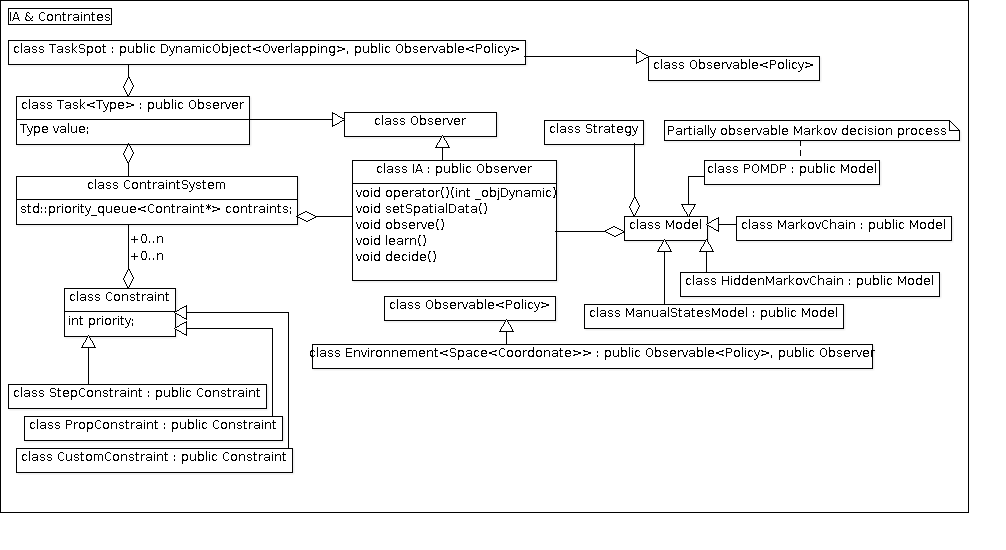
\includegraphics[scale=0.5]{images/c_ia_contraintes.png}
   \caption{\label{c_ia_contraintes} Diagramme de classes d'IA et contraintes}
\end{figure}
